\documentclass[25pt, a0paper, portrait]{tikzposter}
\tikzposterlatexaffectionproofoff

% Set up images
\usepackage{graphicx}
\usepackage{tikz}

% Set up tables
\usepackage{array}
\usepackage{tabularx}
\usepackage{makecell}
\usepackage{multirow}

% Set up links
\usepackage{hyperref}

% Define the center column type
\newcolumntype{C}{>{\centering\arraybackslash}X}%

% set up more math
\usepackage{amsmath}

% Set up bibtex

\usepackage[style=numeric,sorting=none,backend=biber]{biblatex}

\addbibresource{main.bib}

% Customize the title

\title{Classification of Kidney Cortex Cells(COM2028)}
\author{Andre Henriques (6644818)}
\date{\today}
%\institute{University of Surrey}

\definetitlestyle{my-title}{
	roundedcorners=20, linewidth=2pt, innersep=10pt,
	titletotopverticalspace=10mm, titletoblockverticalspace=10mm
}{
	\begin{scope}[line width=\titlelinewidth, rounded corners=\titleroundedcorners]
		\draw[color=blocktitlebgcolor, fill=titlebgcolor, line width=5pt]
		(\titleposleft,\titleposbottom) rectangle (\titleposright,\titlepostop);
	\end{scope}
}
\usetitlestyle{my-title}
\settitle{ \centering
	\color{titlefgcolor} {\bfseries \Huge \sc \@title \par}
	\vspace*{0.2em}
	{\huge \@author \par} \vspace*{0.2em}
}

% Creat the block style

\colorlet{blocktitlefgcolor}{black}

\defineblockstyle{MyBlock}{% define a custom style for a block
    titlewidthscale=0.8, bodywidthscale=1, titlecenter,
    titleoffsetx=0pt, titleoffsety=0pt, bodyoffsetx=0pt, bodyoffsety=15mm,
    bodyverticalshift=15mm, roundedcorners=22, linewidth=5pt,
    titleinnersep=8mm, bodyinnersep=8mm
}{
    \draw[rounded corners=\blockroundedcorners, inner sep=\blockbodyinnersep,
          line width=\blocklinewidth, color=blocktitlebgcolor,
          top color=white, bottom color=white,
          %fill=blockbodybgcolor
          ]
      (blockbody.south west) rectangle (blockbody.north east); %
	    \ifBlockHasTitle%
	        \draw[rounded corners=\blockroundedcorners, inner sep=\blocktitleinnersep,
	          top color=white, bottom color=white,
	          line width=\blocklinewidth, color=blocktitlebgcolor, fill=blocktitlebgcolor
	          ]
	      (blocktitle.south west) rectangle (blocktitle.north east); %
	    \fi%
}

\useblockstyle{MyBlock}


% Other options

\colorlet{backgroundcolor}{white}

\usepackage{comment}

% 
% 
% 
% 
% 
%  Beggining of the text
% 
% 
% 
% 
% 

\begin{document}

\maketitle[roundedcorners=10pt]

%\fontsize{11pt}{15pt}\selectfont

\begin{columns}
	\column{0.3}
% 
% 
% 
% 
% 
% 
	\block{\Large Introduction of the project}{
		\small
		This project attempts to classify images of the human kidney cortex\cite{data, data1} in to 8 distinct categories.
		This dataset is part of the MedMNIST V2\cite{data} dataset of biomedical images that are MNIST\cite{mnist} like.
		As such the the 200 000 images(150000 for training and 50000 for testing) have been formatted as 28 by 28 pixels 
		gray-scale images. The training images will also be split into validation sets and training sets, with a split 
		of $30\%$.\\ 
		As for the expected results, in the original paper\cite{data}, the dataset was tested against various models, 
		with best result obtained, in terms of accuracy, was $70\%$. The objective for this project is to achieve a 
		accuracy over $65\%$ on the testing set. And the final model succeeds in this.
	}
% 
% 
% 
% 
% 
% 
	\block{\Large Analysis of the Problems}{
		\small

		Since this is a machine learning problem there is a need of a library to help us code the models 
		Tensorflow\cite{tensorflow2015-whitepaper} was the chosen for this due to it's simplicity.

		\bigskip

		\textbf{Loading Data:}\\
		The data was given as a folder with all the training images and a .csv file that contains the labels for said
		images. While the data in this format could be loaded using a ImageDataGerator, I decided to learn how 
		tensorflow's dataset system works, and manually load the labels of the images. An example on tensorflow's 
		official documentation shows a base example on how to load loading images manually\cite{tensorflow-images} and
		that example was modified to fit the needs of the project.

		\bigskip

		\textbf{Challenges:}\\
		As with most projects that involve machine learning, computing resources is one of the biggest problems as they
		are limited. My personal computer was used to run the models instead of Googles Colab platform. As there would 
		be no time limitations or timeouts. This does not remove all the limitations as the GPU on my computer only has 
		8 Gigabytes of VRAM which limits the size of the models that can be trained.\\
		\bigskip

		\textbf{Technical issues:}\\
		While the dataset did not have any unusable images the small size of the images and the limited color range 
		limits the amount of information that can be extracted.\\
		It's important to know that some the images have visual artifacts(Fig. \ref{visual atrifacts}) that also limit 
		even more the amount of data that can be extracted from them.\\
		The data set is also not balanced witch makes it harder the model to learn some of the categories of the cells.
		\bigskip

		\begin{tikzfigure}[Images with visual artifacts]
			\label{visual atrifacts}
			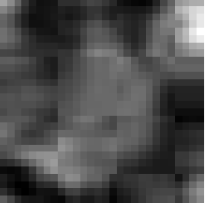
\includegraphics[width=.2\linewidth]{figures/wierd_image_1.png}
			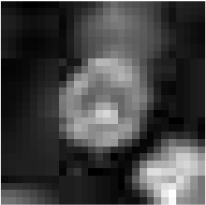
\includegraphics[width=.2\linewidth]{figures/wierd_image_2.png}
		\end{tikzfigure}

		\bigskip
		\textbf {Pre-processing and Overfitting prevention:}\\
		It is also important to add pre-processing before the model so that during training some extra images can be 
		``generated'' that the model can use, this will helps with reducing overfitting.\\
		Therefore all models had a starting data augmentation section.\\
		All models also had dropout layers to prevent overfitting.

		\textbf {Classification techniques:}\\
		There were many classification techniques attempted, the information about it's design and results will be 
		combined into a section about that specific classification method.\\
		The classification methods attempted were:
		\begin {itemize}
			\item 
			Multilayer Perceptron
			\item
			Simple Convolution neural network(CNN)
			\item
			Multi-model Simple CNN
			\item
			Generative Adversarial Network(GAN)
			\item
			Block CNN
		\end {itemize}
	}
% 
% 
% 
% 
% 
% 
	\block{\Large Multilayer Perceptron}{
		\footnotesize
		While multilayer perceptrons\cite{mlp} are not the optimal for the processing the images, the small size of the image 
		makes it possible the use the multilayer perceptrons.\\
		As expected a MLP model did not yield good results with the tested models obtaining around $50\%$ accuracy.
		\begin{tikzfigure}[Results of the MLP]
			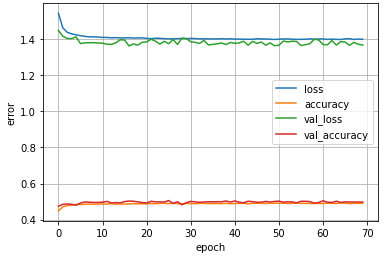
\includegraphics[width=.5\linewidth]{figures/results_mlp.png}
		\end{tikzfigure}
	}
	\block{\Large Simple CNN}{
		\small
		A simple CNN was able to provide better results with less training compared with the the multiplayer perceptron.
		For a CNN that had structure presented in Fig. \ref{simple-CNN} resulted in $61\%$ accuracy, which still leaves
		room for improvement.
		\begin{tikzfigure}[structure of the Simple CNN]
			\label{simple-CNN}
			\resizebox{.6\linewidth}{!}{
				\begin{tabular}{| c | c | c | c | c | c |}
					\hline
					Operation Layer      & Number of filters &  Size of each filter & stride value & padding & size of the output image \\
					Convolution(Conv)    & 64                &  $3\times3$          & $1\times1$   & same    & $28\times28\times64$     \\     
					MaxPooling(Max Pool) & 1                 &  $2\times2$          & $2\times2$   & same    & $14\times14\times64$     \\     
					LeakyRelu            & -                 &  -                   & -            & -       & $14\times14\times64$     \\     
					Dropout              & -                 &  -                   & -            & -       & $14\times14\times64$     \\     
					Conv                 & 128               &  $3\times3$          & $1\times1$   & same    & $14\times14\times128$     \\     
					Max Pool             & 1                 &  $2\times2$          & $2\times2$   & same    & $7\times7\times128$     \\     
					LeakyRelu            & -                 &  -                   & -            & -       & $7\times7\times128$     \\     
					Dropout              & -                 &  -                   & -            & -       & $7\times7\times128$     \\     
					Conv                 & 256               &  $3\times3$          & $1\times1$   & same    & $7\times7\times256$     \\     
					LeakyRelu            & -                 &  -                   & -            & -       & $7\times7\times256$     \\     
					Dropout              & -                 &  -                   & -            & -       & $7\times7\times256$     \\     
					\hline
					Dense layers         &                   &                      &              &         &                          \\     
					\hline
				\end{tabular}
			}
		\end{tikzfigure}
		\begin{tikzfigure}[Results of the Simple CNN]
			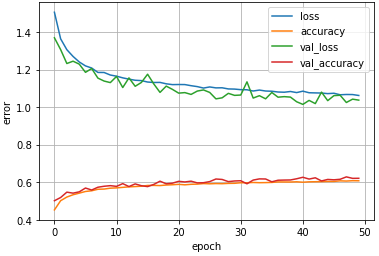
\includegraphics[width=.5\linewidth]{figures/simple_cnn.png}
		\end{tikzfigure}
	}
	\column{0.7}
	\begin{subcolumns}
		\subcolumn{0.5}
		\block{Multi Model CNN}{
			\normalsize		
			The Multi Model CNN is very similar to the single model approach, but in this case each category was given a 
			model. That model was trained to only recognize that specific cell type. \\
			Each model was trained individually, when there is a need to predict, all models are presented with the same 
			image, and the type is decided by measuring which model is more confident on the image being it's type.\\
			In the end this model had similar results to the simple CNN, with overall smaller models, but an increase in 
			the total training time, as the number of models to train also increased.

			\begin{tikzfigure}[Structure of each of the models used by the multimodel approach]
				\resizebox{\linewidth}{!}{
					\begin{tabular}{| c | c | c | c | c | c |}
						\hline
						Operation Layer      & Number of filters &  Size of each filter & stride value & padding & size of the output image \\
						Convolution(Conv)    & 64                &  $3\times3$          & $1\times1$   & same    & $28\times28\times64$     \\     
						MaxPooling(Max Pool) & 1                 &  $2\times2$          & $2\times2$   & same    & $14\times14\times64$     \\     
						LeakyRelu            & -                 &  -                   & -            & -       & $14\times14\times64$     \\     
						Dropout              & -                 &  -                   & -            & -       & $14\times14\times64$     \\     
						Conv                 & 128               &  $3\times3$          & $1\times1$   & same    & $14\times14\times128$    \\     
						Max Pool             & 1                 &  $2\times2$          & $2\times2$   & same    & $7\times7\times128$      \\     
						LeakyRelu            & -                 &  -                   & -            & -       & $7\times7\times128$      \\     
						Dropout              & -                 &  -                   & -            & -       & $7\times7\times128$      \\     
						\hline
						Dense layers         &                   &                      &              &         &                          \\     
						\hline
					\end{tabular}
				}
			\end{tikzfigure}
			\begin{tikzfigure}[Results of some of the models]
				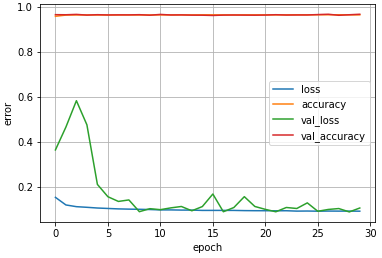
\includegraphics[width=.4\linewidth]{figures/multi_cnn_1.png}
				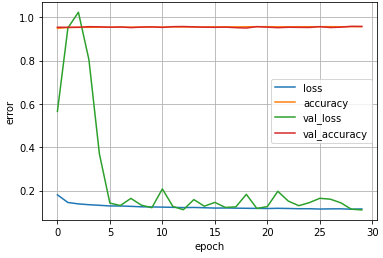
\includegraphics[width=.4\linewidth]{figures/multi_cnn_2.png}
			\end{tikzfigure}
		}
		\subcolumn{0.5}
		\block{GAN}{
			\normalsize		

			GAN\cite{gan} are created by having 2 models a discriminator and generator. The generator tries to create 
			new images based on the dataset and the discriminator tries to tell the difference between the generated 
			images and the real ones. The loss of the discriminator is based on how good is the generator at recognizing 
			the differences between the generated image and the real one, and so it's the generators. In the best case, 
			both the generator and the discriminator get incredibly effective at generating/discriminating images.

			The generator and the discriminator were modified so that the they would take into account type of the cells 
			that the original image had.

			Unfortunately the generator model did not converge and the images that where generated, where not good 
			enough for this method to be effective.

			The overall accuracy ended up being around $30\%$.

			After the last model was created I discovered that the average pool function is better for this images and 
			which means that generator model could have converged if they were used instead of the Max pooling layers 
			that were used.

			\vspace*{.5em}

			\begin{tikzfigure}[Failed generated images]
				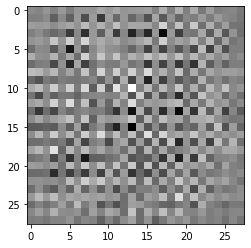
\includegraphics[width=.3\linewidth]{figures/fail_image.png}
				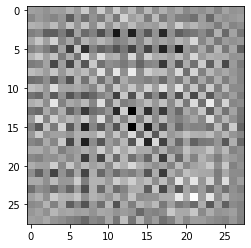
\includegraphics[width=.3\linewidth]{figures/fail_image_2.png}
			\end{tikzfigure}

			\vspace*{.509em}
		}
	\end{subcolumns}	
	\block{\Large Block CNN}{
		\normalsize
		The Block CNN is formed a group of blocks(defined in Fig. \ref{tab:structure-block}), the blocks contain a group 
		of convolution layers separated with ReLU activation functions. Each block ends with a batch normalization, 
		a pooling, a LeakyReLU, and a Dropout layers.\\
		This design was chosen do to many tests, where the value accuracy and tested for improvements, and the bests
		techniques where selected.\\
		The AdamW optimizer was chosen as it helps with reducing overfitting\cite{adamw}.
		\smallskip
		Average pooling was found to be more suited for this kind of images as they don't have hard edges which benefit
		more from Max pooling.\\
		\smallskip
		As a final optimization this model was not loaded the images as 28 by 28 images but 32 by 32 upscaled images, as 
		it provided more data to the model witch tends improve performance. After the model was build the model was run
		but with gamma corrected images\cite{gamma_correction_1} which also improved performance.
		\begin{tikzfigure}[Structure of each block]
			\label{tab:structure-block}
			\resizebox{.64\linewidth}{!}{
				\begin{tabular}{| c | c | c | c | c | c |}
					\hline
					Operation Layer      & Number of filters &  Size of each filter & stride value                            & padding                      & size of the output image \\
					\hline
					Conv                 & number of filters &  Size of each filter & $1\times1$                              & same                         & \multirow{2}{*}{$\text{Input}_x\times\text{Input}_y\times\text{Number of filters}$}\\
					ReLu                 & -                 &  -                   & -                                       & -                            & \\     
					\hline
					(block size times)   &                   &                      &                                         &                              &                                                                    \\     
					\hline
					Batch Normalization  & -                 &  -                   & -                                       & -                            & \multirow{4}{*}{\shortstack{$\text{Input}_x\times\text{Input}_y\times\text{Number of filters}$\\ or\\ $\frac{\text{Input}_x}{2}\times\frac{\text{Input}_y}{2}\times\text{Number of filters}$}}\\ 
					Pooling Function     & 1                 &  $2\times2$          & \makecell{$2\times2$\\ or\\ $1\times1$} & \makecell{valid\\ or\\ same} & \\
					LeakyRelu            & -                 &  -                   & -                                       & -                            & \\
					Dropout              & -                 &  -                   & -                                       & -                            & \\
					\hline
				\end{tabular}
			}
		\end{tikzfigure}

		Then this sets of this blocks are used to create the full network.

		\begin{tikzfigure}[Structure of the network]
			\label{best-of-best}
			\resizebox{.64\linewidth}{!}{
				\begin{tabular}{| c | c | c | c | c | c | c |}
					\hline
					Operation Layer & Size of The block & Number of filters &  Size of each filter & padding & Pooling function & size of the output image \\
					\hline
					Block           & 1                 & 64                &  1                   & same    & Average          & $32\times32\times64$     \\     
					Block           & 2                 & 128               &  3                   & valid   & Average          & $16\times16\times128$    \\     
					Block           & 2                 & 250               &  3                   & valid   & Average          & $8\times8\times250$      \\     
					Block           & 2                 & 500               &  3                   & valid   & Average          & $4\times4\times500$      \\     
					Block           & 1                 & 1000              &  3                   & same    & Average          & $4\times4\times1000$     \\     
					\hline
					Global Average  &                   &                   &                      &         &                  &                          \\                
					\hline
				\end{tabular}
			}
		\end{tikzfigure}

		The first block is used as a way to increase the number of channels of the input image without the increase the 
		big computational overhead due to the 1 by 1 filter, the same way it's used by ResNet\cite{resnet}.\\

		Global average Pooling proved to be better than using dense layers, which is supported by other studies dealing 
		with the classification other biomedical issues\cite{brain-cell-class, breast-cell-class}. And and this case the
		model with global average pooling (Fig. \ref{global}) outperformed the one without global average pooling (Fig.
		\ref{no-global}).\\

		A deeper(same structure but bigger block sizes) model, then the one shown in Fig. \ref{best-of-best} without gamma correction was able to get an accuracy 
		score of $66.8\%$, while this smaller model was able to $67.23\%$.

		\begin{minipage}[t]{.25\linewidth}
			\begin{tikzfigure}[Results with larger model and without global average; gamma correction]
				\label{no-global}
				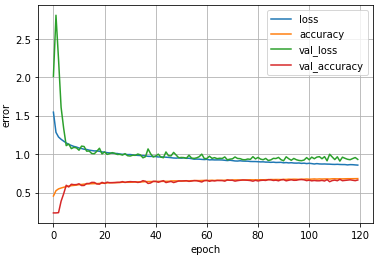
\includegraphics[width=.8\linewidth]{figures/block_cnn.png}
			\end{tikzfigure}
		\end{minipage}
		\begin{minipage}[t]{.25\linewidth}
			\begin{tikzfigure}[Results with larger model and without: gamma correction]
				\label{global}
				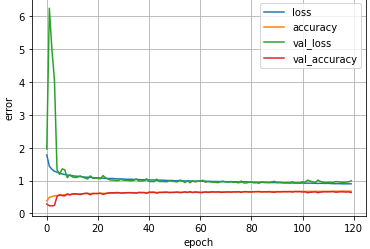
\includegraphics[width=.8\linewidth]{figures/block_cnn_better.png}
			\end{tikzfigure}
		\end{minipage}
		\begin{minipage}[t]{.25\linewidth}
			\begin{tikzfigure}[Final results]
				\label{global}
				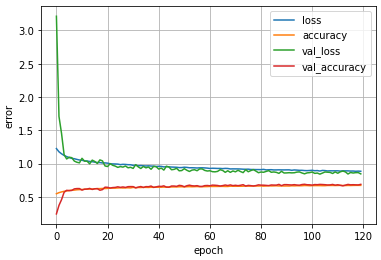
\includegraphics[width=.84\linewidth]{figures/block_cnn_better_gamma.png}
			\end{tikzfigure}
		\end{minipage}
		\begin{minipage}[t]{.25\linewidth}
			\begin{tikzfigure}[Gamma corrected cell]
				\label{global}
				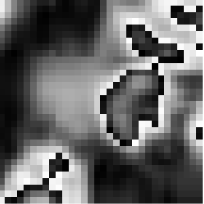
\includegraphics[width=.53\linewidth]{figures/gamma_addjusted.png}
			\end{tikzfigure}
		\end{minipage}
	}
	\block{\Large Results}{
		\small
		As it was mention before the model that resulted in better accuracy scores was the Block CNN model. \\
		But this does not mean that it is the best model. I expect if the block CNN was applied with a multi model
		approach it would out perform the main base block CNN model.\\
		Machine learning could also be used to train the hyper parameters of the model, as it was done with the
		original paper\cite{data}, with a tool like AutoKeras\cite{autokeras}.\\
		Since we only can submit one notebook, but more models were created the rest of the models can be found
		in this GitHub repository: \url{https://github.com/andr3h3nriqu3s11/COM2028-other-models}
		\vspace{1.2em}
	}
	\block[bodyinnersep=17pt]{\large References}{
		\AtNextBibliography{\tiny}
		\printbibliography[heading=none]
	}
\end{columns}

\end{document}